\documentclass[12pt]{amsart}
\usepackage{geometry} % see geometry.pdf on how to lay out the page. There's lots.
\usepackage{graphicx}	% Including figure files
\usepackage{amsmath}	% Advanced maths commands
\usepackage{amssymb}	% Extra maths symbols
\usepackage{hyperref}
\usepackage{float}
\floatplacement{figure}{H}
\floatplacement{table}{H} 
\geometry{a4paper} % or letter or a5paper or ... etc

\title{CSE 546: Machine Learning Homework 4}
\author{David P. Fleming}
\date{December 12th, 2016}

%%% BEGIN DOCUMENT
\begin{document}

\maketitle
\tableofcontents

\section*{Introduction}

Please note that a copy of all the code I wrote to answer the questions in this assignment are included in my submission but also located online at \url{https://github.com/dflemin3/CSE_546/tree/master/HW4}.  Some scripts require data, such as MNIST data, to run to completion and were not included on my github due to file size constraints.  

Overall, my code is structured as follows:  There are three main directories included in my submission: {\tt DML}, {\tt Data} and {\tt HW4}. {\tt HW4} contains all the scripts used to run my analysis.  For example to reproduce the answer for Question 2.1, one would run {\tt python hw4$\_2.1.py$}.  All scripts have relative file paths so the code should run and have detailed comments to describe functionality.  In addition, the scripts have flags near the top to control functionality.  By default, I set all flags to true so the script performs the entire analysis and plotting.  

The {\tt DML} directory contains all the auxiliary files used to do the computations in the homework scripts and has a logical hierarchy.  For example, the directory {\tt optimization} contains the file {\tt gradient$\_$descent.py} while contains both my batch gradient descent and stochastic gradient descent implementations.  The directory {\tt data$\_$processing} contains the script {\tt mnist$\_$utils.py} which contains my functions used to load and work with the MNIST data.  The directory {\tt classification} contains the file {\tt classifier$\_$utils.py} which contains all things related to binary and softmax classification including the gradients for each respective method for use with a gradient descent algorithm.  The {\tt validation} subdirectory contains {\tt validation.py}.  This file contains all my loss functions such as 0/1 loss and also my implementations for regularization paths for both linear regression and logistic and softmax classification using gradient descent.  The {\tt deep$\_$learning} directory contains all neural network functionality.  Finally, the {\tt regression} directory contains all utilities for a normal or multi-class regression.  In each section, I try to be explicit with what files I used to perform the computation including the path from the {\tt DML} directory for ease of grading.

%%% QUESTION 0  %%%
\section*{Question 0: Collaborators}
I collaborated with Matt Wilde, Serena Liu, and Janet Matsen for various questions on this assignment.

%%% QUESTION 1 %%%
\section*{Question 1: Manual calculation of one round of EM for a GMM}
Here I perform one round of EM for a GMM on the 1D data $x = [1,10,20]$.  All M and E step equations are taken from Murphy section 11.4.2.

\subsection*{1.1: M step}
\subsubsection*{1.1.1}
The likelihood function we optimize is taken Murphy (eqn. 11.26) and is
\begin{equation}
\sum_i \sum_c R_{ic} \log \pi_c + \sum_i \sum_c R_{ic} \log p(x_i | \theta_c).
\end{equation}
\subsubsection*{1.1.2}
The M step to update $\pi$ is 
\begin{equation}
\pi_c = \frac{1}{N} \sum_i R_{ic}.
\end{equation}
Applying this equation to the given data gives the updated mixing weights
\begin{equation}
\pi_1 = \frac{1 + 0.4}{3} = 0.467
\end{equation}
and 
\begin{equation}
\pi_2 = \frac{0.6 + 1}{3} = 0.533.
\end{equation}

\subsubsection*{1.1.3}
The M step for the means is
\begin{equation}
\mu_c = \frac{\sum_i R_{ic x_i}}{R_c}.
\end{equation}
Apply this equation to the given data gives the updated means
\begin{equation}
\mu_1 = \frac{(1 \cdot 1) + (10 \cdot 0.4) + (20 \cdot 0)}{1.4} = 3.57
\end{equation}
and
\begin{equation}
\mu_2 = \frac{(0 \cdot 1) + (10 \cdot 0.6) + (20 \cdot 1)}{1.6} = 16.25.
\end{equation}

\subsubsection*{1.1.4}
The M step for the standard deviation is
\begin{equation}
\Sigma_c = \frac{\sum_i R_{ic}(x_i - \mu_c)(x_i - \mu_c)^T}{R_c}
\end{equation}
where $\sigma_c = \sqrt{\Sigma_c}$ for the 1D case.  Applying this equation to the given data gives the updated standard deviations
\begin{equation}
\sigma_1 = \sqrt{\frac{1(1-3.57)^2 + 0.4(10-3.57)^2}{1.4}} = 4.07
\end{equation}
and
\begin{equation}
\sigma_2 = \sqrt{\frac{0.6(10-16.25)^2 + 1(20-16.25)^2}{1.6}} = 4.84.
\end{equation}

\subsection*{1.2: E Step}

\subsubsection*{1.2.1}
The probability for observation $x_i$ belonging to cluster $c$ is the responsibility
\begin{equation}
R_{ic} = \frac{\pi_c p(x_i | \theta_c^{(t-1)})}{\sum_{c'}\pi_{c'} p(x_i | \theta_{c'}^{(t-1)})}
\end{equation}
where $p(x_i | \theta_c^{(t-1)}) = N(\mu_c,\sigma_c)$ for the assumed GMM.

\subsubsection*{1.2.2}
After performing the E step, the new value of R is
\begin{equation}
R = 
\begin{pmatrix}
    0.99  & 0.01 \\
    0.41  & 0.59 \\
    0       & 1      \\
\end{pmatrix}
\end{equation}
where the last row values barely changed ($< 1 \times 10^{-4}$) in this iteration.

%%% QUESTION 2 %%%
\section{Question 2: Neural Nets and Backprop}
The code used for this question is given in {\tt hw4$\_$2.1.py, hw4$\_$2.2.py, hw4$\_$2.3.py} in the {\tt DML} directory and uses my neural network routines found in the file {\tt deep$\_$utils.py} in the directory {\tt deep$\_$learning}.

For all parts of this question and for computational speed purposes, I first performed dimension reduction using PCA.  I fit my PCA algorithm on the MNIST training set and then projected each image using the first $k = 50$ components.  I did not subtract off the mean when fitting for PCA as the mean component swamped out the differences between the hidden layer weights images.  

I used mini-batch SGD with a mini-batch size of 10 for all gradient calculations during the backprop step.  Each half epoch, or each complete pass through half of the randomly permuted training set, I performed 30,000/10 = 3,000 mini-batch gradient updates.  I computed the square loss of the entire transformed training set and testing set (to which I applied the same transformation as the training set for consistency).  I called my algorithm converged either once the mean square loss on the training set did not change by more than $0.01\%$ or when the algorithm has passed through the training set a certain number of times, typically 25.  Since this is a non-convex optimization problem, I found that once near convergence, the loss jumped around substantially necessitating terminating the optimization after a certain number of epochs.  I did not explicitly use regularization since the early-stopping from the combination of my capped number of epochs and my learning rate decay scheme (described below) implicitly $l_2$ regularize my solution.  I used this exact same optimization scheme for both Questions 2.2 and 2.3 (see below).  Interestingly, I found that the same learning rate and scaling parameter yielded optimal performances for all my solutions as shown below.

My testing set 0/1 loss to beat for a comparable neural network architecture from the official MNIST website is $4.5\%$ for a 2-layer neural network with 1000 hidden units.  

\subsection*{2.1: With tanh hidden units}
For this question I optimized a 2-layer neural network with tanh hidden units and a linear output layer.  I used one-against-all classification to predict the digit label.

\subsubsection*{2.1.1}
I used a learning rate $\eta = 1 \times 10^{-3}$.  In practice in my SGD implementation at the start of each epoch, I reset $\eta = k\eta_0/N$ where $N$ is the number of samples in a batch, $k = 1/\sqrt{t}$ is a scaling constant where $t$ is the epoch number and $\eta_0 = 1 \times 10^{-3}$.  I found that decaying the weights allowed the solution to achieve better results while minimizing how much the loss bounces around.   As stated above, I used a mini-batch size of 10.  For this problem, I capped the maximum number of passes through the training set for my SGD mini-batch optimization at 50.

I initialized the weights which map the input to the hidden layer by randomly sampling from $N(0,\sigma)$ for each element of the $d \times n_{nodes}$ weight matrix where I computed 
\begin{equation}
\sigma = \frac{c}{||X||^2_2}
\end{equation}
for $d$ features in the dataset.  I set the arbitrary scaling constant $c = 0.001$ to keep the weights near zero to prevent from the solution from getting stuck in the flat part of the tanh function.  I initial the second $n_{nodes} \times n_{classes}$ weight matrix which maps the hidden layer to the output layer by randomly sampling from $N(0,\sigma)$ for each element of the weight matrix where I computed 
\begin{equation}
\sigma = \frac{c}{\sqrt{n_{nodes}}}
\end{equation}
where $n_{nodes}$ is the number of nodes in the hidden layer and I set $c = 0.001$ as justified above.

\subsubsection*{2.1.2}
I plot square loss as a function of half epoch in Fig.~\ref{fig:tanh_linear_sq} and the 0/1 loss as a function of half epoch in Fig.~\ref{fig:tanh_linear_01}.  I only plot the 0/1 loss once it has dipped below $7\%$ for readability.
\begin{figure}[H]
	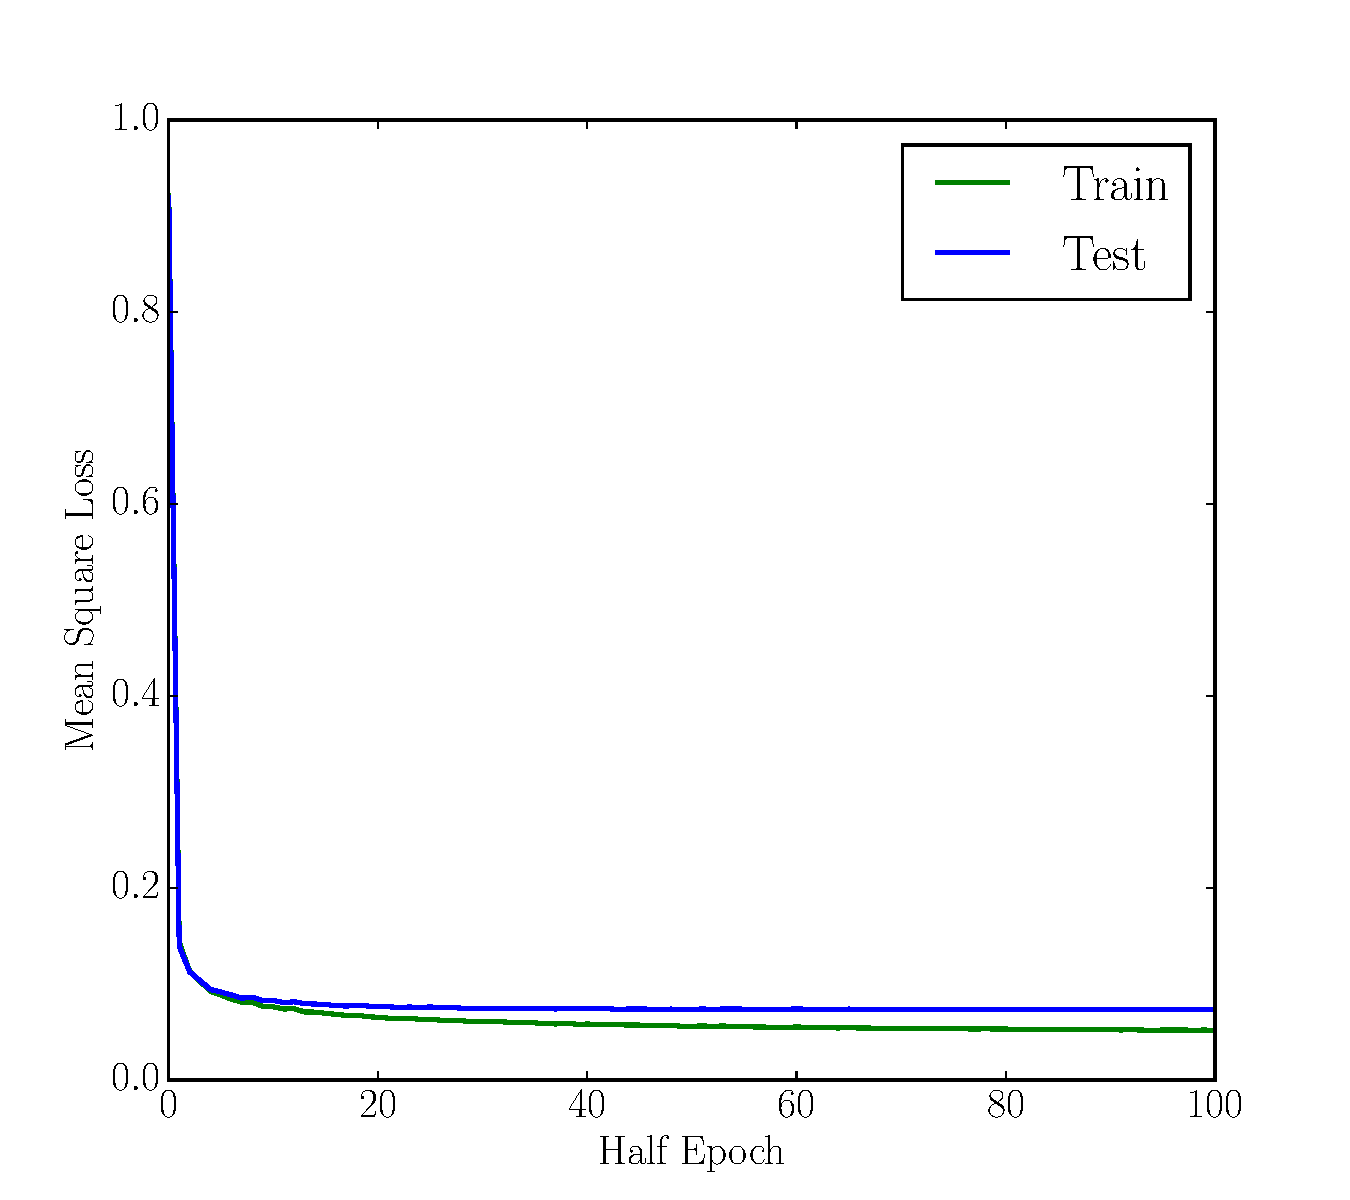
\includegraphics[width=\columnwidth]{tanh_linear_sq.pdf}
    \caption{Square loss for both the training and testing sets as a function of half epochs for a 2 layer neural network with a tanh hidden unit and linear output units.}
    \label{fig:tanh_linear_sq}
\end{figure}
\begin{figure}[H]
	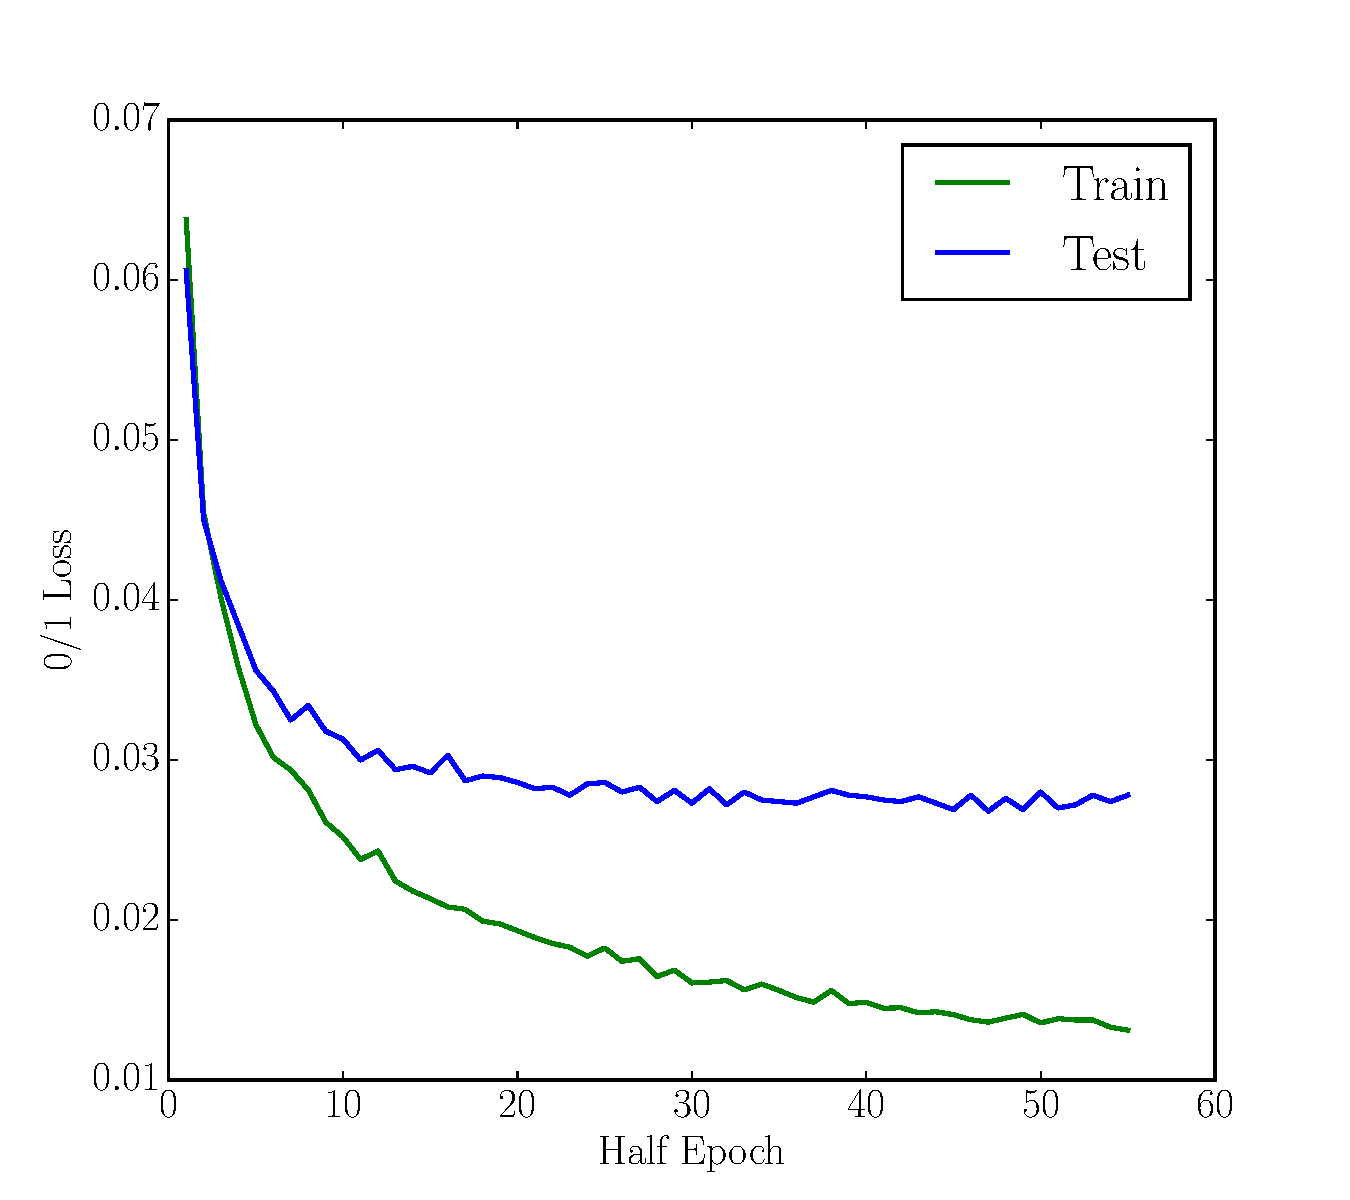
\includegraphics[width=\columnwidth]{tanh_linear_01.pdf}
    \caption{0/1 loss for both the training and testing sets as a function of half epochs for a 2 layer neural network with a tanh hidden unit and linear output units.}
    \label{fig:tanh_linear_01}
\end{figure}
In the first few epoch, both the square and 0/1 losses for both the training and testing sets drop dramatically.  Although the square loss seems to slowly asymptote until the maximum number of iterators, the 0/1 losses decay but noticeably bounce around due to the non-convex nature of this optimization.  As expected, the training 0/1 loss continues to decay as I train on the training set but the testing loss seems to bottom-out indicating that running SGD for more epochs would only lead to over-fitting.

\subsubsection*{2.1.3}
My final squared losses on the training and testing sets are 0.051509 and 0.073138, respectively.  My final 0/1 losses on the training and testing sets are 0.010933 and 0.026500, respectively.  My performance on the testing set for this architecture and set of activation functions is much better than the MNIST website benchmark.

\subsubsection*{2.1.4}
In Fig.~\ref{fig:tanh_linear_hidden}, I choose 10 hidden layer nodes at random and display the learned weights projected back into image space.
\begin{figure}[H]
	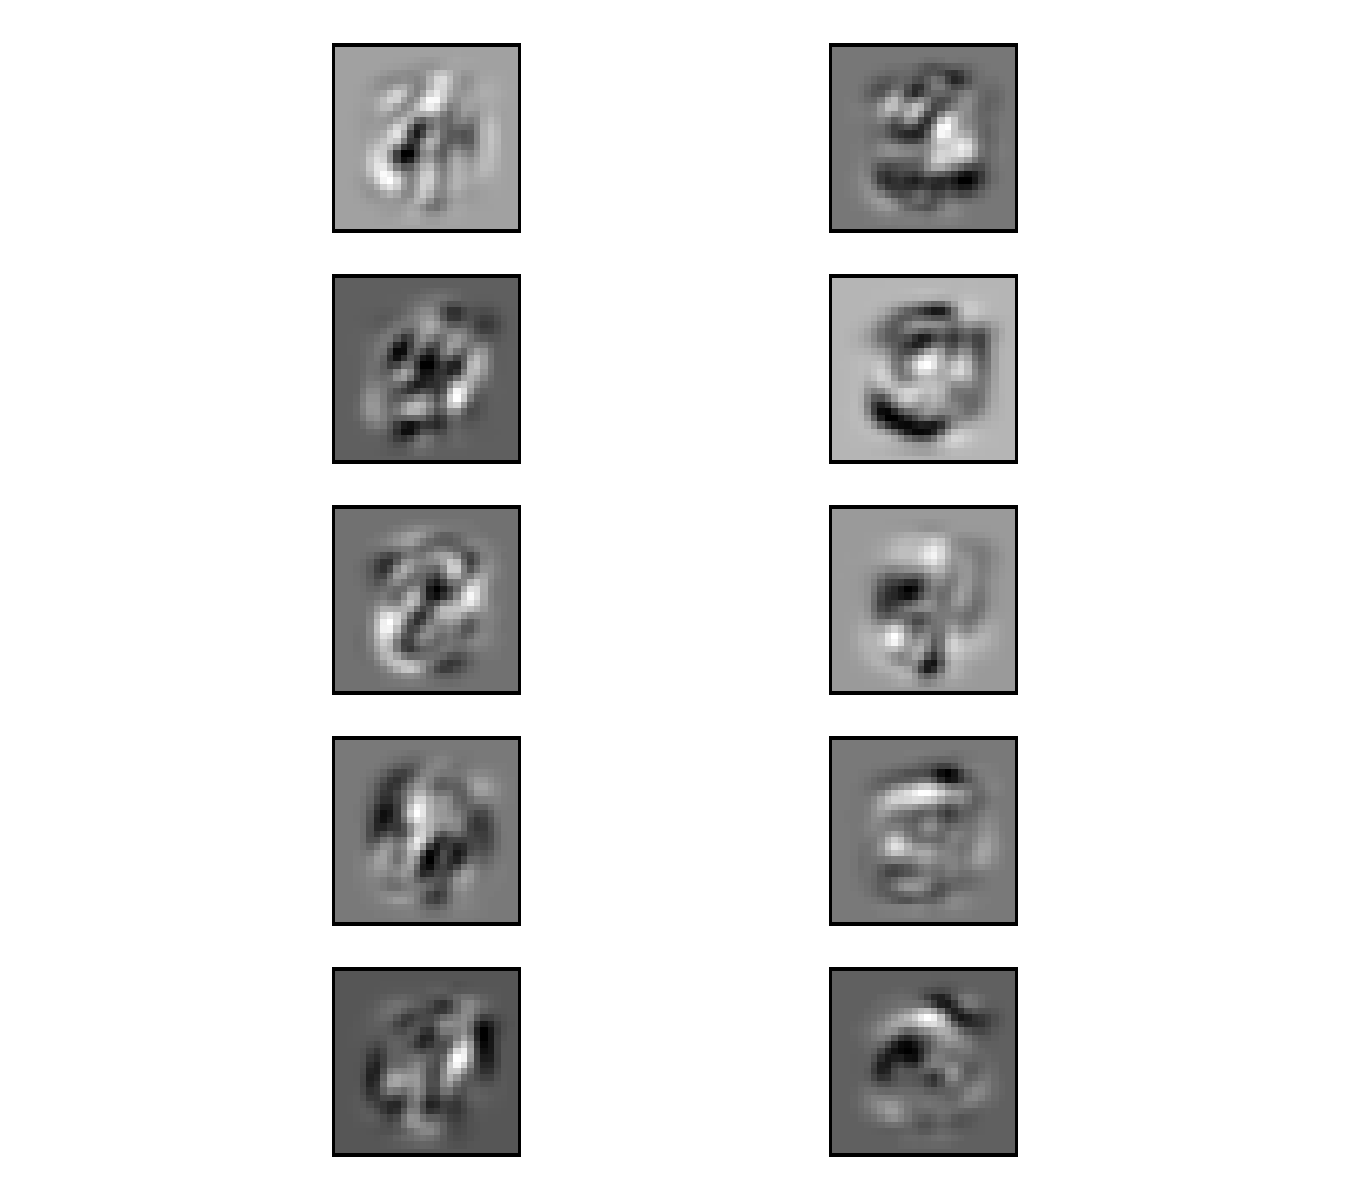
\includegraphics[width=\columnwidth]{tanh_linear_hidden.pdf}
    \caption{10 randomly sampled hidden layer weights reprojected into the original image space for a 2 layer neural network with a tanh hidden unit and linear output units.}
    \label{fig:tanh_linear_hidden}
\end{figure}
All the hidden weights appear to be seemingly random combinations of digits with additional noisy jitter.

\subsection*{2.2: With ReLu hidden units}
For this question I optimized a 2-layer neural network with ReLu hidden units and a linear output layer.  I used one-against-all classification to predict the digit label.

\subsubsection*{2.2.1}
I used a learning rate $\eta = 1 \times 10^{-3}$.  In practice in my SGD implementation at the start of each epoch, I reset $\eta = k\eta_0/N$ where $N$ is the number of samples in a batch, $k = 1/\sqrt{t}$ is a scaling constant where $t$ is the epoch number and $\eta_0 = 1 \times 10^{-3}$.  I found that decaying the weights allowed the solution to achieve better results while minimizing how much the loss bounces around.   As stated above, I used a mini-batch size of 10.  For this problem, I capped the maximum number of passes through the training set for my SGD mini-batch optimization at 25.

I initialized the weights which map the input to the hidden layer by randomly sampling from $N(0,\sigma)$ for each element of the $d \times n_{nodes}$ weight matrix where I computed 
\begin{equation}
\sigma = \frac{c}{||X||^2_2}
\end{equation}
for $d$ features in the dataset.  I set the arbitrary scaling constant $c = 0.001$ to keep the weights near zero to prevent from the solution from blowing up when the weights are far from 0.  I initial the second $n_{nodes} \times n_{classes}$ weight matrix which maps the hidden layer to the output layer by randomly sampling from $N(0,\sigma)$ for each element of the weight matrix where I computed 
\begin{equation}
\sigma = \frac{c}{\sqrt{n_{nodes}}}
\end{equation}
where $n_{nodes}$ is the number of nodes in the hidden layer and I set $c = 0.001$ as justified above.

\subsubsection*{2.2.2}
I plot square loss as a function of half epoch in Fig.~\ref{fig:relu_linear_sq} and the 0/1 loss as a function of half epoch in Fig.~\ref{fig:relu_linear_01}.  I only plot the 0/1 loss once it has dipped below $7\%$ for readability.
\begin{figure}[H]
	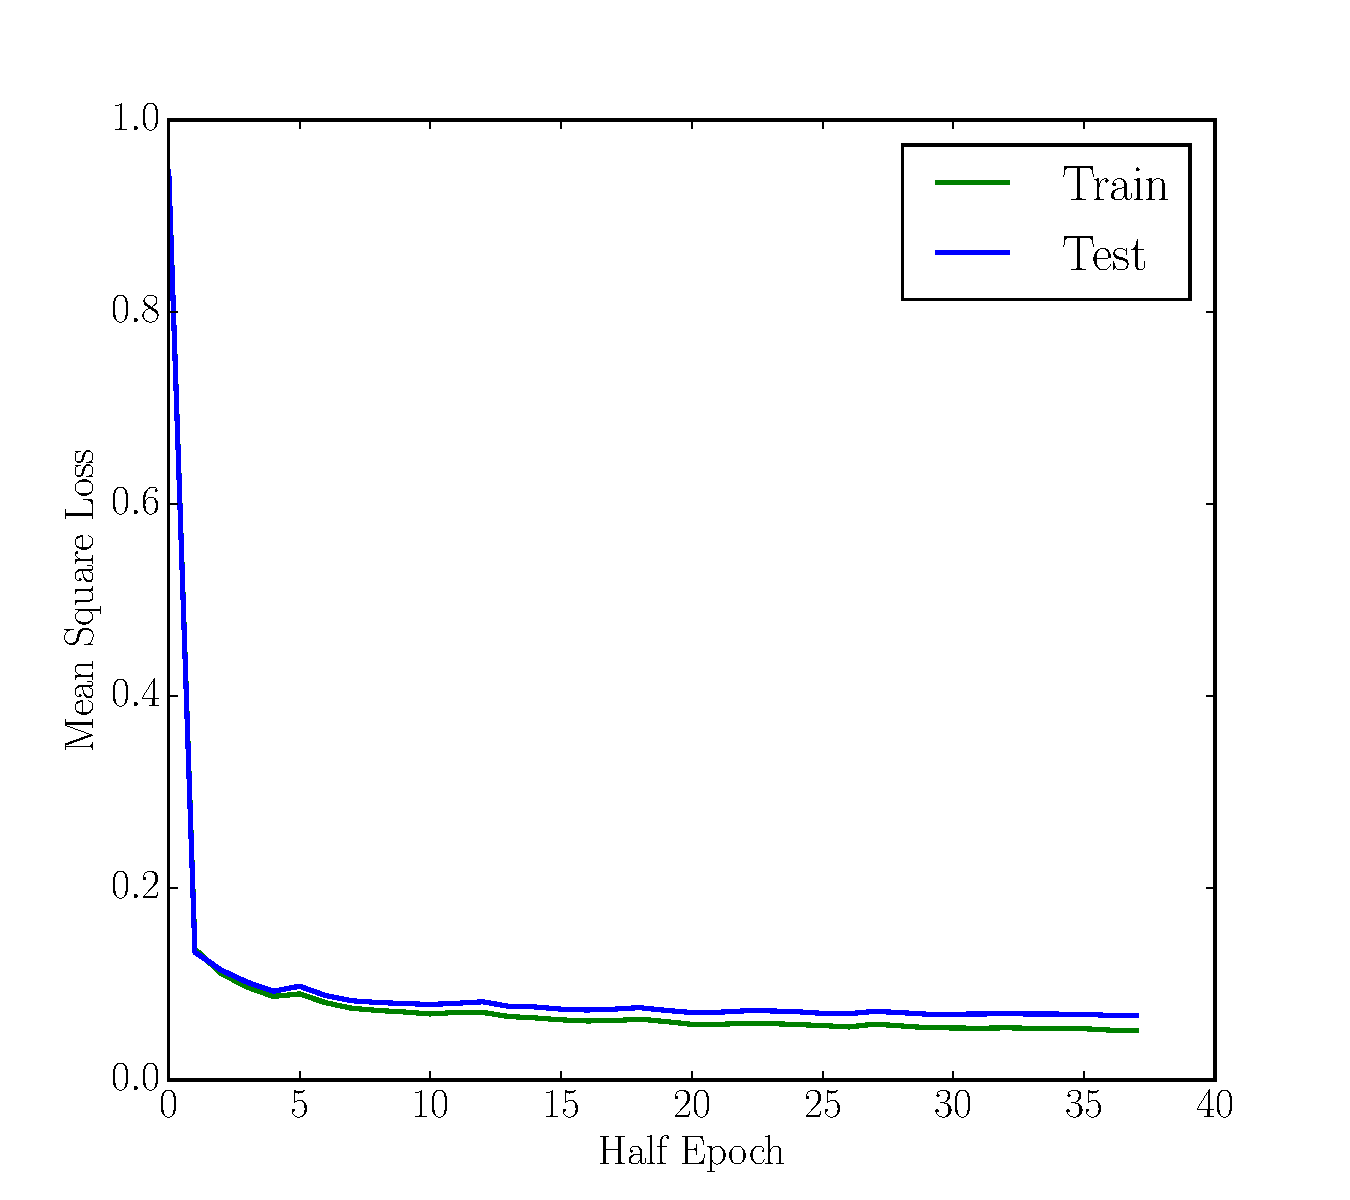
\includegraphics[width=\columnwidth]{relu_linear_sq.pdf}
    \caption{Square loss for both the training and testing sets as a function of half epochs for a 2 layer neural network with a ReLu hidden unit and linear output units.}
    \label{fig:relu_linear_sq}
\end{figure}
\begin{figure}[H]
	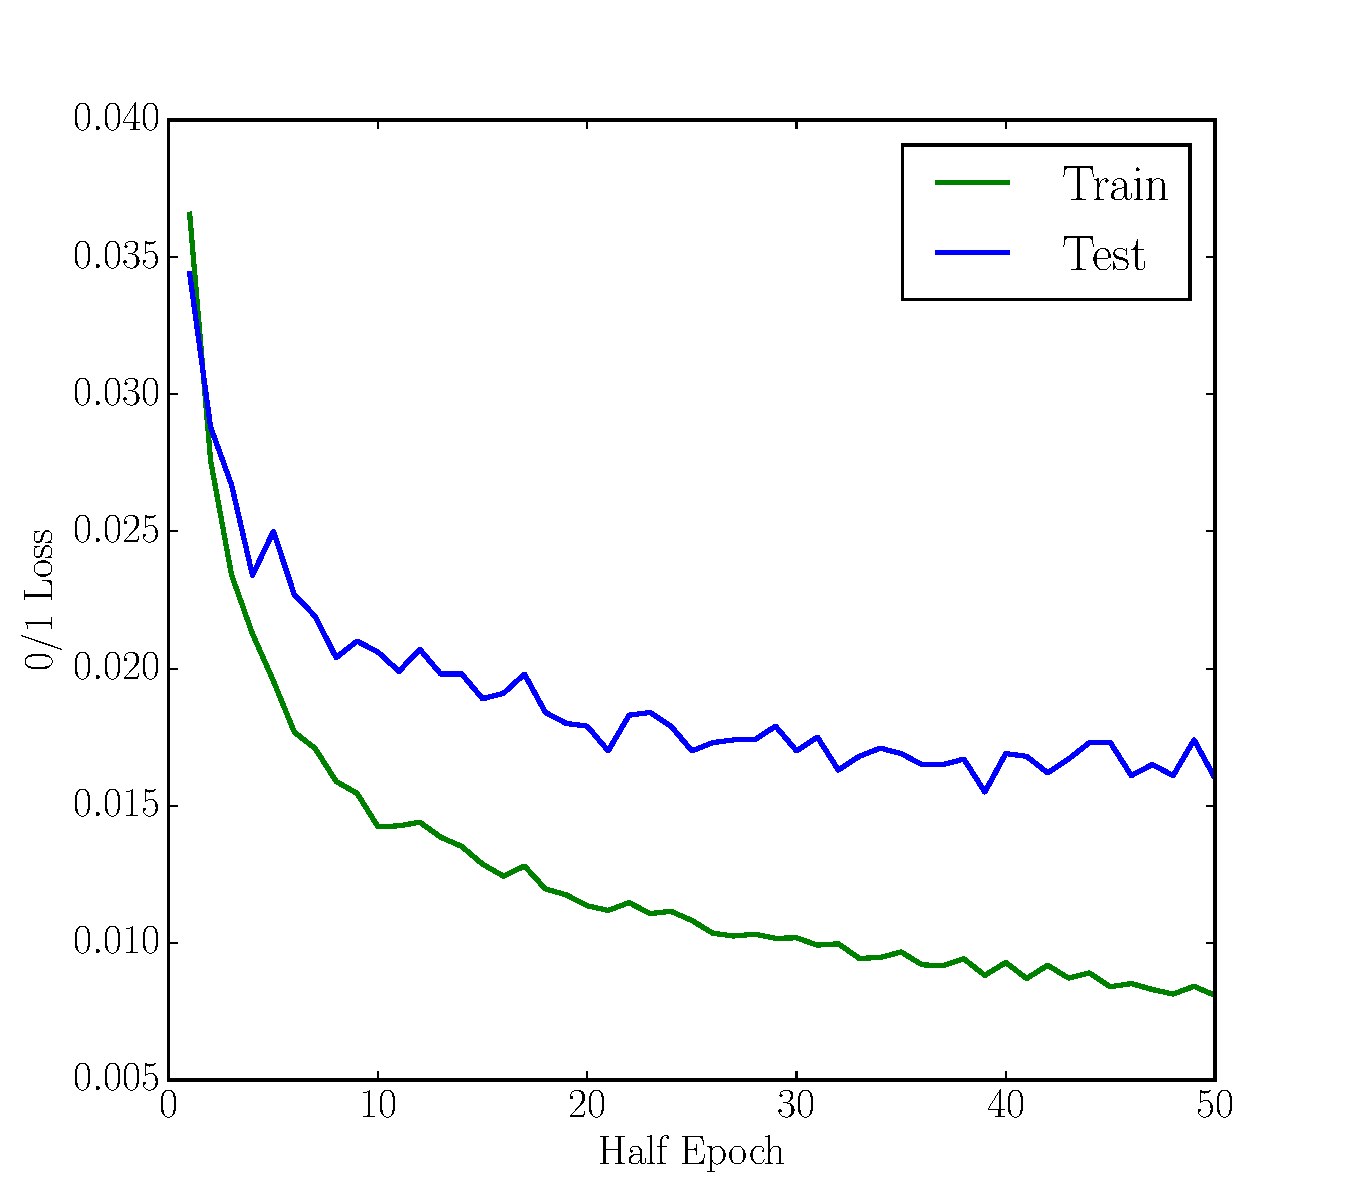
\includegraphics[width=\columnwidth]{relu_linear_01.pdf}
    \caption{0/1 loss for both the training and testing sets as a function of half epochs for a 2 layer neural network with a ReLu hidden unit and linear output units.}
    \label{fig:relu_linear_01}
\end{figure}
In the first few epoch, both the square and 0/1 losses for both the training and testing sets drop dramatically.  Although the square loss seems to slowly asymptote until the maximum number of iterators, the 0/1 losses decay but substantially bounce around, much more so than for the tanh hidden unit optimization.  This additional stochastic bouncing is likely due to the piece-wise linear nature of the ReLu function and its non-continuos derivative.  As expected, the training 0/1 loss continues to decay as I train on the training set but the testing loss seems to bottom-out indicating that running SGD for more epochs would only lead to over-fitting.

\subsubsection*{2.2.3}
My final squared losses on the training and testing sets are 0.049179 and 0.065924, respectively.  My final 0/1 losses on the training and testing sets are 0.008083 and 0.016000, respectively.  My performance on the testing set for this architecture and set of activation functions is much better than the MNIST website benchmark and than my tanh activation function solution.  It is interesting that learning with a simple nonlinear function like ReLu yields substantially better performance than the tanh layer with much fewer iterations.

\subsubsection*{2.2.4}
In Fig.~\ref{fig:relu_linear_hidden}, I choose 10 hidden layer nodes at random and display the learned weights projected back into image space.
\begin{figure}[H]
	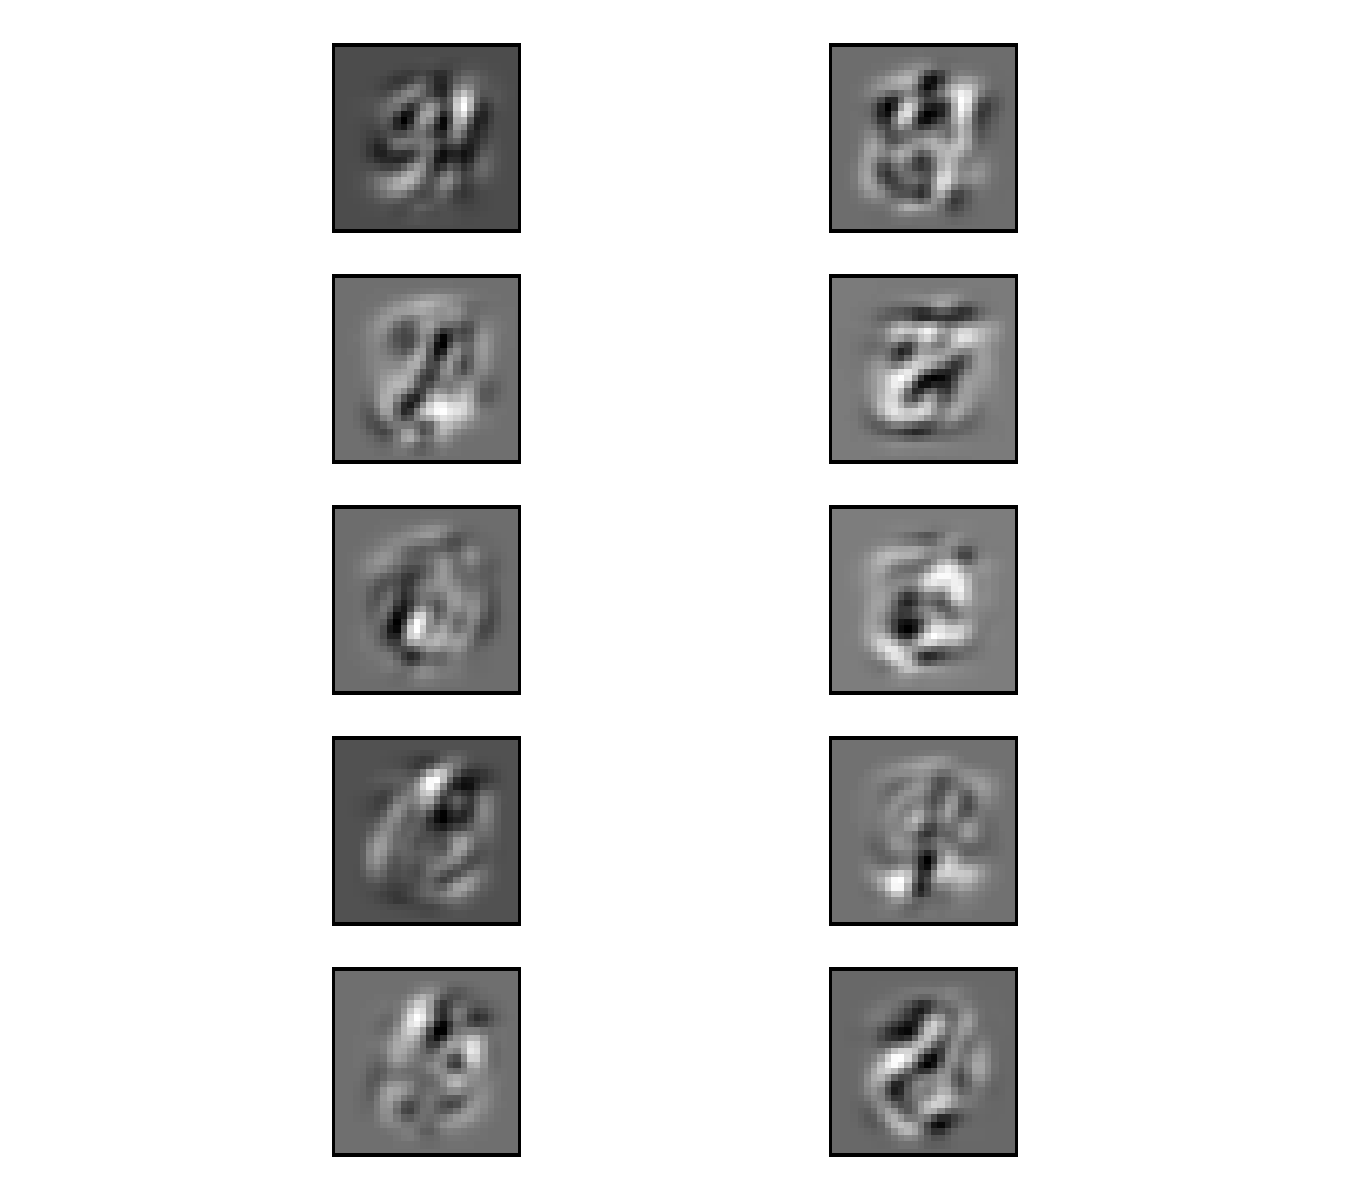
\includegraphics[width=\columnwidth]{relu_linear_hidden.pdf}
    \caption{10 randomly sampled hidden layer weights reprojected into the original image space for a 2 layer neural network with a ReLu hidden unit and linear output units.}
    \label{fig:relu_linear_hidden}
\end{figure}
All the hidden weights appear to be seemingly random combinations of digits with additional noisy jitter as before.

\subsection*{2.3: With ReLu hidden units + ReLu output units}
For this question I optimized a 2-layer neural network with ReLu hidden units and a ReLu output layer.  I used one-against-all classification to predict the digit label.

\subsubsection*{2.3.1}
I used a learning rate $\eta = 1 \times 10^{-3}$.  In practice in my SGD implementation at the start of each epoch, I reset $\eta = k\eta_0/N$ where $N$ is the number of samples in a batch, $k = 1/\sqrt{t}$ is a scaling constant where $t$ is the epoch number and $\eta_0 = 1 \times 10^{-3}$.  I found that decaying the weights allowed the solution to achieve better results while minimizing how much the loss bounces around.   As stated above, I used a mini-batch size of 10.  For this problem, I capped the maximum number of passes through half of the training set for my SGD mini-batch optimization at 75.

I initialized the weights which map the input to the hidden layer by randomly sampling from $N(0,\sigma)$ for each element of the $d \times n_{nodes}$ weight matrix where I computed 
\begin{equation}
\sigma = \frac{c}{||X||^2_2}
\end{equation}
for $d$ features in the dataset.  I set the arbitrary scaling constant $c = 0.001$ to keep the weights near zero to prevent from the solution from blowing up when weights are far from 0.  I initial the second $n_{nodes} \times n_{classes}$ weight matrix which maps the hidden layer to the output layer by randomly sampling from $N(0,\sigma)$ for each element of the weight matrix where I computed 
\begin{equation}
\sigma = \frac{c}{\sqrt{n_{nodes}}}
\end{equation}
where $n_{nodes}$ is the number of nodes in the hidden layer and I set $c = 0.001$ as justified above.

\subsubsection*{2.3.2}
I plot square loss as a function of half epoch in Fig.~\ref{fig:relu_relu_sq} and the 0/1 loss as a function of half epoch in Fig.~\ref{fig:relu_relu_01}.  I only plot the 0/1 loss once it has dipped below $7\%$ for readability.
\begin{figure}[H]
	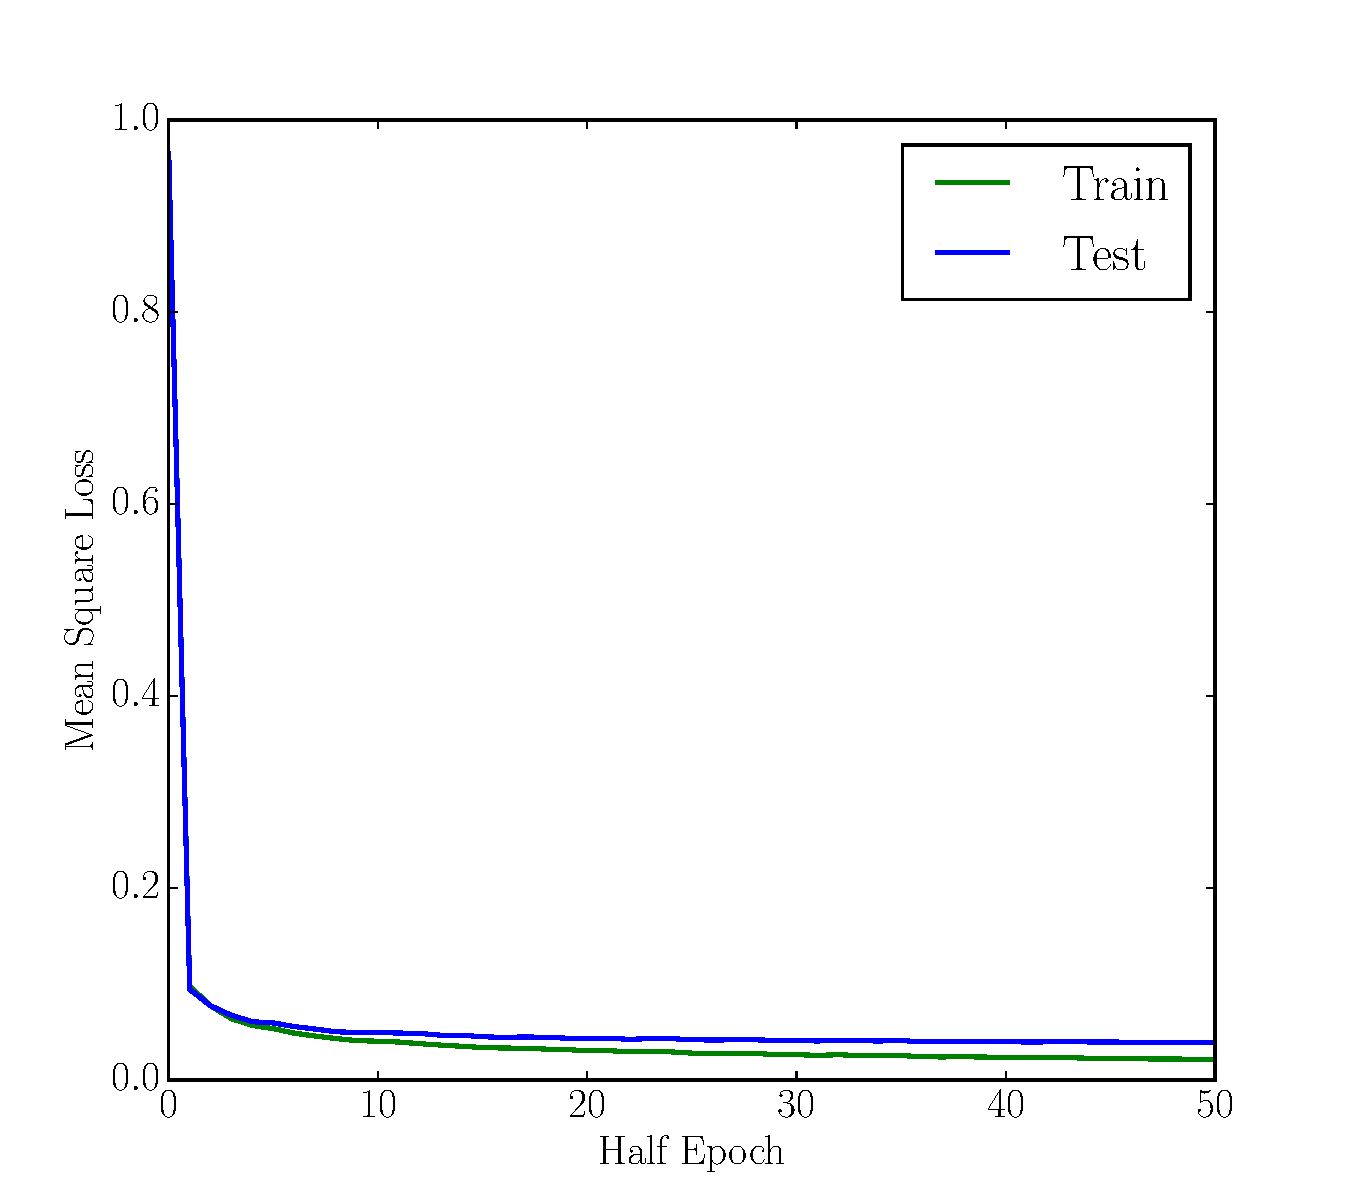
\includegraphics[width=\columnwidth]{relu_relu_sq.pdf}
    \caption{Square loss for both the training and testing sets as a function of half epochs for a 2 layer neural network with a ReLu hidden unit and ReLu output units.}
    \label{fig:relu_relu_sq}
\end{figure}
\begin{figure}[H]
	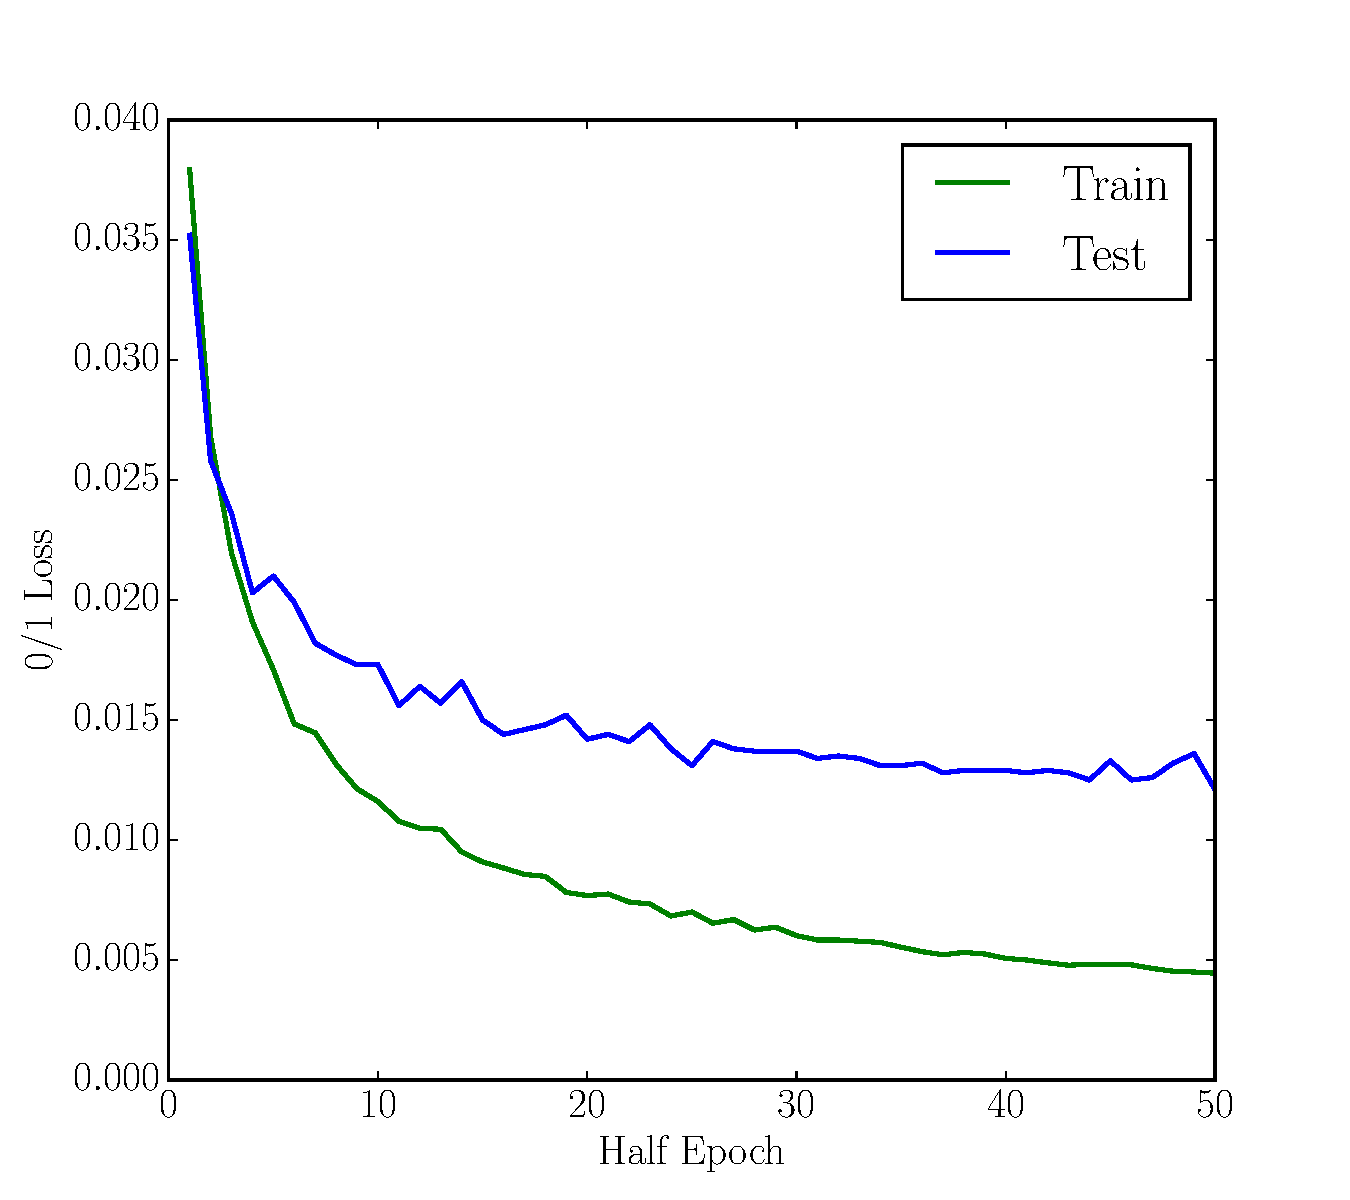
\includegraphics[width=\columnwidth]{relu_relu_01.pdf}
    \caption{0/1 loss for both the training and testing sets as a function of half epochs for a 2 layer neural network with a ReLu hidden unit and ReLu output units.}
    \label{fig:relu_relu_01}
\end{figure}
As before, both the square and 0/1 losses decrease dramatically after one pass through the training set and then slowly bounce down towards a local minima.  As expected and seen in the previous two questions, the testing loss is greater than the training loss.

\subsubsection*{2.3.3}
My final squared losses on the training and testing sets are 0.014006 and 0.037826, respectively.  My final 0/1 losses on the training and testing sets are 0.003017 and 0.012400, respectively.  My performance on the testing set for this architecture and set of activation functions is substantially better than the MNIST website benchmark much better than my other solutions.  It is fascinating how using simple ReLu layers can yield such excellent performance.

\subsubsection*{2.3.4}
In Fig.~\ref{fig:relu_relu_hidden}, I choose 10 hidden layer nodes at random and display the learned weights projected back into image space.
\begin{figure}[H]
	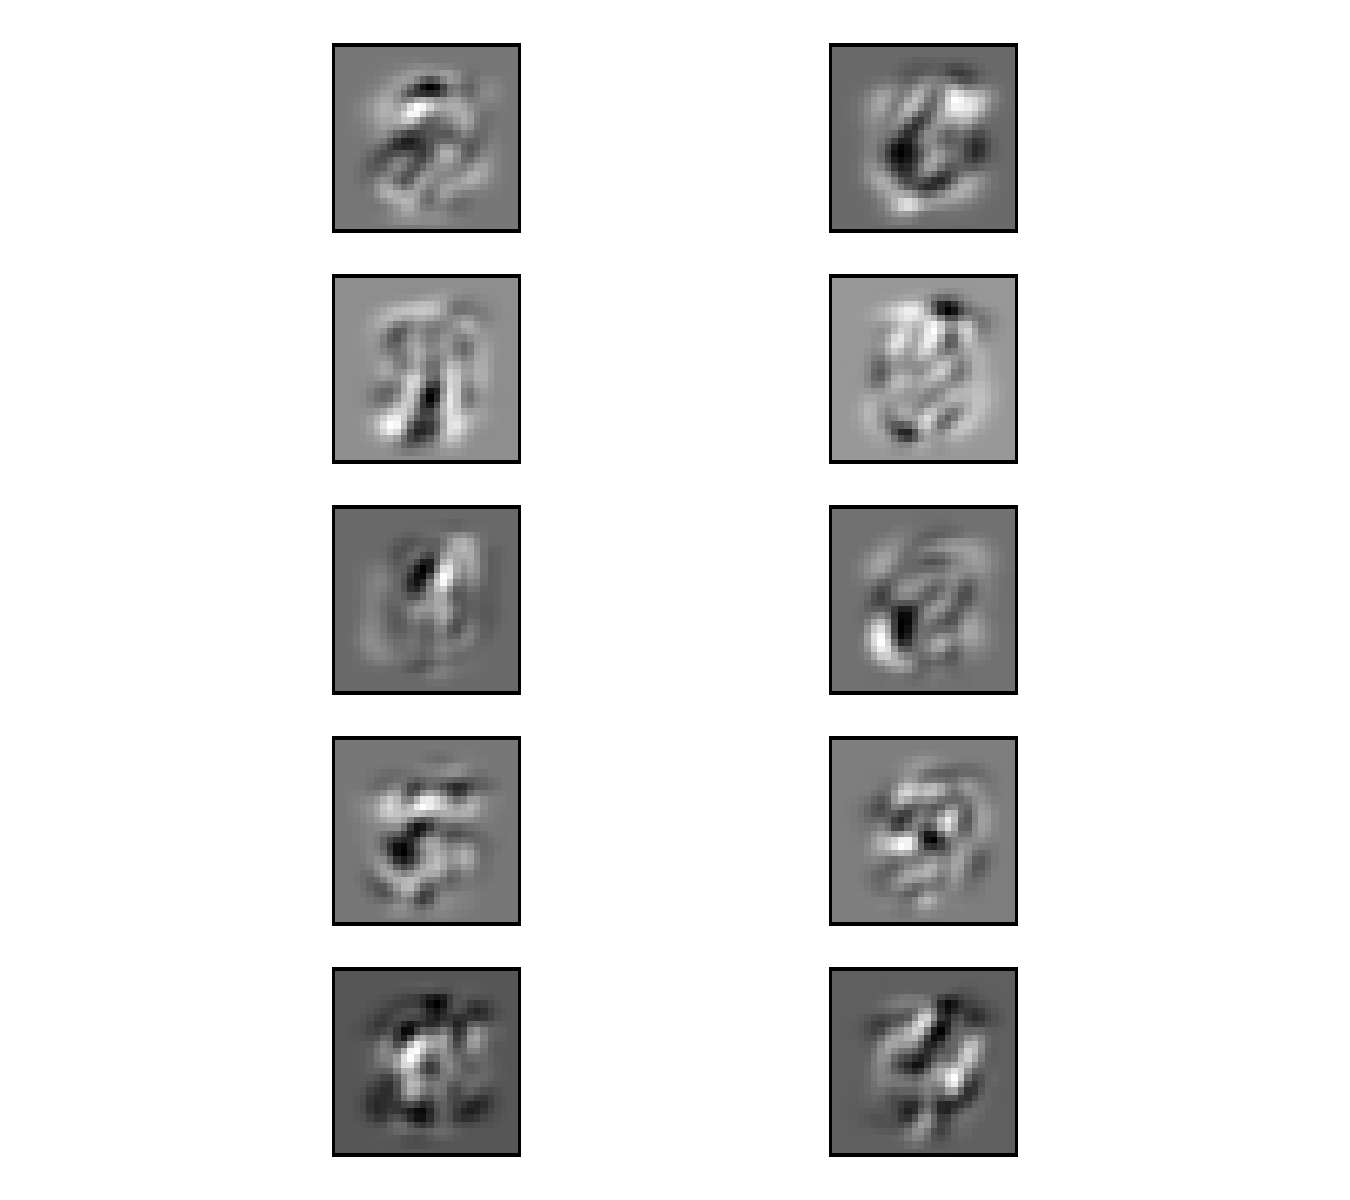
\includegraphics[width=\columnwidth]{relu_relu_hidden.pdf}
    \caption{10 randomly sampled hidden layer weights reprojected into the original image space for a 2 layer neural network with a ReLu hidden unit and ReLu output units.}
    \label{fig:relu_relu_hidden}
\end{figure}
As before, all the hidden weights appear to be seemingly random combinations of digits with additional noisy jitter.

\section*{3: EM v.s. Gradient Descent}

\subsection*{3.1}
I will show that
\begin{equation}
\nabla L(\theta) = E_{Z {\sim}P(z|x,\theta)} \nabla \log P(x,z|\theta)
\end{equation}
and note that I will use the relation
\begin{equation} \label{eqn:bayes_3}
P(z|x,\theta)P(x|\theta) = P(x,z|\theta).
\end{equation}

I expand the gradient of the likelihood to get
\begin{equation}
\begin{split}
\nabla L(\theta) & = \frac{\partial}{\partial \theta} \log P(x|\theta) \\
& \frac{1}{P(x|\theta)} \frac{\partial}{\partial \theta} P(x|\theta) \\
& \frac{1}{P(x|\theta)} \frac{\partial}{\partial \theta} \sum_z P(x, z|\theta) \\
& =  \frac{1}{P(x|\theta)} \sum_z  \frac{\partial}{\partial \theta} P(x, z|\theta) \\
& = \sum_z  \frac{1}{P(x|\theta)}  \frac{\partial}{\partial \theta} P(x, z|\theta) \\
& = \sum_z  \frac{P(z|x,\theta)}{P(x,z|\theta)}  \frac{\partial}{\partial \theta} P(x, z|\theta) \\
&= \sum_z P(z|x,\theta) \nabla \log P(x,z|\theta) \\
& =  E_{Z {\sim}P(z|x,\theta)} \nabla \log P(x,z|\theta)
\end{split}
\end{equation}
where I made use of Eqn.~\ref{eqn:bayes_3} to replace $1/P(x|\theta)$, completing the proof.

\subsection*{3.2}
Alice and Bob are doing the same thing since at that point, the gradient of the loss function and the gradient of the product of the E step are identical.  In the E step, we compute the expected complete data log likelihood via the auxiliary function, Q, where the expectation is taken with respect to the old parameters and the observed data.  Therefore at that same point, the gradient of the expected log likelihood is equal to the gradient of the true log likelihood so a gradient descent update on either Q or the true log likelihood will be equivalent.

\subsection*{3.3}
If ran to convergence, the EM algorithm reaches a critical point, either a local optimum or a saddle point, where the gradient of the log likelihood function is 0.  This occurs because EM monotonically increases the observed data log likelihood until it reaches a local optimum.  After the E step, the expected complete log likelihood is a tight lower bound to the log likelihood function so any maximization on this lower bound, via the M step, is assured to update the model parameters to increase the observed data log likelihood until reaching a local optimum.  Specifically in therms of the expected complete data log likelihood $Q$ and log likelihood $l$, we have
\begin{equation}
l(\theta^{t+1}) \geq Q(\theta^{t+1},\theta^{t}) \geq Q(\theta^{t+1},\theta^{t}) = l(\theta^{t}) 
\end{equation}
so when $l(\theta^{t+1}) = l(\theta^{t})$, $Q(\theta^{t+1},\theta^{t}) = Q(\theta^{t+1},\theta^{t})$ and the algorithm has converged to a local optimum.

\section*{4: Markov Decision Processes and Dynamic Programming}
TODO

\subsection*{4.1}
TODO

\subsection*{4.2}
TODO

\subsection*{4.3}
TODO

\end{document}




















